\documentclass{standalone}

\usepackage{tikz}
\usepackage{tkz-euclide}

\usepackage{times}

\usetikzlibrary{positioning}
\usetikzlibrary{arrows.meta}

\definecolor{accent}{rgb}{0.9,0.9,0.9}

\begin{document}
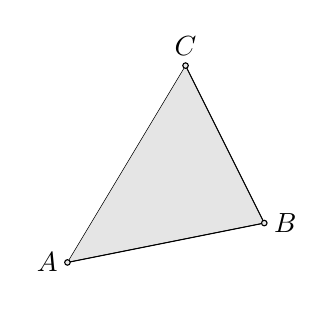
\begin{tikzpicture}

  \tkzDefPoint(-1.0,-0.8){min}
  \tkzDefPoint(3.0,3.0){max}

  \tkzDefPoint(0,0){A}
  \tkzDefPoint(2.5,0.5){B}
  \tkzDefPoint(1.5,2.5){C}

  \draw[draw,fill=accent] (A)--(B)--(C);
  \tkzDrawSegments(A,B B,C C,A)
  \tkzDrawPoint(A)
  \tkzDrawPoint(B)
  \tkzDrawPoint(C)

  \tkzLabelPoints[right](B)
  \tkzLabelPoints[above](C)
  \tkzLabelPoints[left](A)

\end{tikzpicture}
\end{document}
